\documentclass[10pt,leter,openany]{article}
\usepackage[latin1]{inputenc}
\usepackage[english]{babel}
\usepackage{amsmath}
\usepackage{amsfonts}
\usepackage{amssymb}
\usepackage{graphicx}
\usepackage{listings}
\usepackage{color}
\usepackage[left=3cm,right=3cm,top=3cm,bottom=3cm]{geometry}
\usepackage[numbers,sort&compress]{natbib}
\usepackage{url}
\usepackage{caption}
\usepackage{siunitx}
%\usepackage{subfigure}
\usepackage{float}
\usepackage{booktabs}
\usepackage{subcaption}
\usepackage{comment}
\usepackage{mwe}
%\usepackage[table,xcdraw]{xcolor}

\setlength{\parindent}{0pt}
\setlength{\parskip}{4pt}

\definecolor{mygreen}{rgb}{0,0.6,0}
\definecolor{mygray}{rgb}{0.5,0.5,0.5}
\definecolor{mymauve}{rgb}{0.58,0,0.82}

\lstset{ 
	backgroundcolor=\color{white},   % choose the background color; you must add \usepackage{color} or \usepackage{xcolor}; should come as last argument
	basicstyle=\footnotesize,        % the size of the fonts that are used for the code
	breakatwhitespace=false,         % sets if automatic breaks should only happen at whitespace
	breaklines=true,                 % sets automatic line breaking
	captionpos=b,                    % sets the caption-position to bottom
	commentstyle=\color{mygreen},    % comment style
	deletekeywords={...},            % if you want to delete keywords from the given language
	escapeinside={\%*}{*)},          % if you want to add LaTeX within your code
	extendedchars=true,              % lets you use non-ASCII characters; for 8-bits encodings only, does not work with UTF-8
	firstnumber=01,                	 % start line enumeration with line 1000
	frame=single,	                 % adds a frame around the code
	keepspaces=true,                 % keeps spaces in text, useful for keeping indentation of code (possibly needs columns=flexible)
	keywordstyle=\color{blue},       % keyword style
	language=Python,                 % the language of the code
	morekeywords={*,...},            % if you want to add more keywords to the set
	numbers=left,                    % where to put the line-numbers; possible values are (none, left, right)
	numbersep=5pt,                   % how far the line-numbers are from the code
	numberstyle=\tiny\color{mygray}, % the style that is used for the line-numbers
	rulecolor=\color{black},         % if not set, the frame-color may be changed on line-breaks within not-black text (e.g. comments (green here))
	showspaces=false,                % show spaces everywhere adding particular underscores; it overrides 'showstringspaces'
	showstringspaces=false,          % underline spaces within strings only
	showtabs=false,                  % show tabs within strings adding particular underscores
	stepnumber=1,                    % the step between two line-numbers. If it's 1, each line will be numbered
	stringstyle=\color{mymauve},     % string literal style
	tabsize=2,	                     % sets default tabsize to 2 spaces
	title=\lstname                   % show the filename of files included with \lstinputlisting; also try caption instead of title
}

\usepackage[dvipsnames,table,xcdraw]{xcolor}

\usepackage{fancyvrb}

% redefine \VerbatimInput
\RecustomVerbatimCommand{\VerbatimInput}{VerbatimInput}%
{fontsize=\footnotesize,
	%
	frame=lines,  % top and bottom rule only
	framesep=2em, % separation between frame and text
	rulecolor=\color{Gray},
	%
	label=\fbox{\color{Black}data.txt},
	labelposition=topline,
	%
	commandchars=\|\(\), % escape character and argument delimiters for
	% commands within the verbatim
	%commentchar=*        % comment character
}



\usepackage{titling}
\newcommand{\subtitle}[1]{%
	\posttitle{%
		\par\end{center}
	\begin{center}\large#1\end{center}
	\vskip0.5em}%
}


\author{5273}
\title{Homework Assignment 7: Applied Probabilistic Models}
\subtitle{Curve Fitting}
\date{}


\begin{document}
	
\maketitle

\section{Introduction}
	
	Fitting a distribution from a dataset consists of finding the parameters' value, which, with greater probability, that distribution could have generated the observed data \citep{joaquin2020}. For example, the normal distribution has two parameters (mean and variance); once these two parameters are known, the entire distribution is known.
	
	For the analysis, the R software is used in its version 4.0.2 \citep{r}, and the code used is available on the GitHub repository of  \citep{github}. This work is run on a MacBook Air with an Intel Core i5 CPU $ @ $ 1.8 GHz and 8 GB RAM.
	
	
	\section{Data}
	
	For this work, four functions have been created. Independent variables $x_{1}, x_{2}$ are the result of generated values using the R function \texttt{runif()}, $x_{3}$ is generated by the function \texttt{rchisq()} with two degrees of freedom, and $ x_{4} $, using \texttt{rnorm} with its defuault values of mean 0 and standard deviation of 1.
	
		\begin{equation} \label{eq:1}
				y =4x_{1} + 5x_{2},
		\end{equation}  
		
		\begin{equation} \label{eq:2}
				 y = (x_{1})^{2} + \texttt{rexp(1)},
			\end{equation}  
		
	%	\begin{equation} \label{eq:3}
	%			  y_{1} = \sqrt{x_{a}}+1, \hspace{0.1cm} y_{2} = 2x_{2} + \texttt{rnorm(1)},
	%		\end{equation}  
		
		\begin{equation} \label{eq:4}
				y = e^{2}(x_{1})^{2}(x_{2}) ^{3} ,
			\end{equation}  
		
		\begin{equation} \label{eq:5}
			y = (4x_{1})^{3}(20x_{2}) + \dfrac{x_{3}}{5} + \log (x_{4})^{2} .
		\end{equation}  
	
	
	In real case scenarios, the relation of the variables is unknown most of the time, meaning that a model that best describes this relation has to be found.


\section{Experiments}

	The experiments for this work are based on the generated functions described in the previous section. The parameter used is the number of repetitions or sample size ($n$), with a value of 100. The previous functions are used in the transformations described in this report and analyzed one of them in each section of the experiments.

	\subsection{Multiple Linear Regression}

		For the Function \ref{eq:1}, and assuming that the relationship between variables is unknown, it is considered to find the parameters or coefficient that best described this relation. In this case, it could be useful to perform a regression analysis.

		\VerbatimInput{extras/linear_regression_eq1.txt}

		Regression in R software can be performed with the \texttt{lm()} function, which can be obtained the coefficients that best described a relation given by the form $ Y = \beta_{1} + \beta_{2}X + \epsilon$ \citep{selva2016}. In this case, lets assume that it is known that function $y$  depends on $x_{1}$ and $x_{2}$. For this reason, a multiple linear regression analysis is needed. This is an extension of simple linear regression used to predict an outcome variable ($y$) based on multiple distinct predictor variables ($x$). With two predictor variables ($x$), the prediction of $y$ is expressed by the  equation $ Y = \beta_{0} + \beta_{1}X_{1} + \beta_{2}X_{2}$ \citep{kassambara2018}. Once the experiment is performed it throws in the column ``Estimate" of the R output these $\beta$ coefficients. In this case $\beta_{1}=4$ and $\beta_{2}=5$ which corresponds to the values previously declared when generating the function. The intercept value correspond with an error when estimate this relation.

	\subsection{Box-Cox Transformation}
	
		In some cases, if assumptions of the simplicity of structure for $E(y)$), the constancy of error variance and normality of distributions are not satisfied in terms of the original observations, a non-linear transformation of $y$ may improve the analysis \citep{box1964analysis}.  Box-Cox transformation is given by the equation:


		\begin{equation}
			y^{\lambda}= \left\{ \begin{array}{lcc}
				\dfrac{y^{\lambda}-1}{\lambda} &   if  & \lambda \neq 0, \\
				\\ \log y &  if & \lambda = 0. \\
			\end{array}
			\right.
		\end{equation}

		Figure \ref{fig:lr_df2} show plots of the diagnosis of  function \ref{eq:2}, fitting a model without doing a transformation first. The ``Residual vs Fitted" plot shows a more concentrate residual points between  0 and -1 lines. The ``Quantile-Quantile" plot shows the normality of the errors, and it is not great specially at the upper tail, which goes off from the straight line. The ``Scale-Location" plot, which shows there is no homoscedasticity and the ``Residuals vs. Leverage" plot which shows if there are outliers in the residuals.

		\begin{figure}
			\begin{center}
				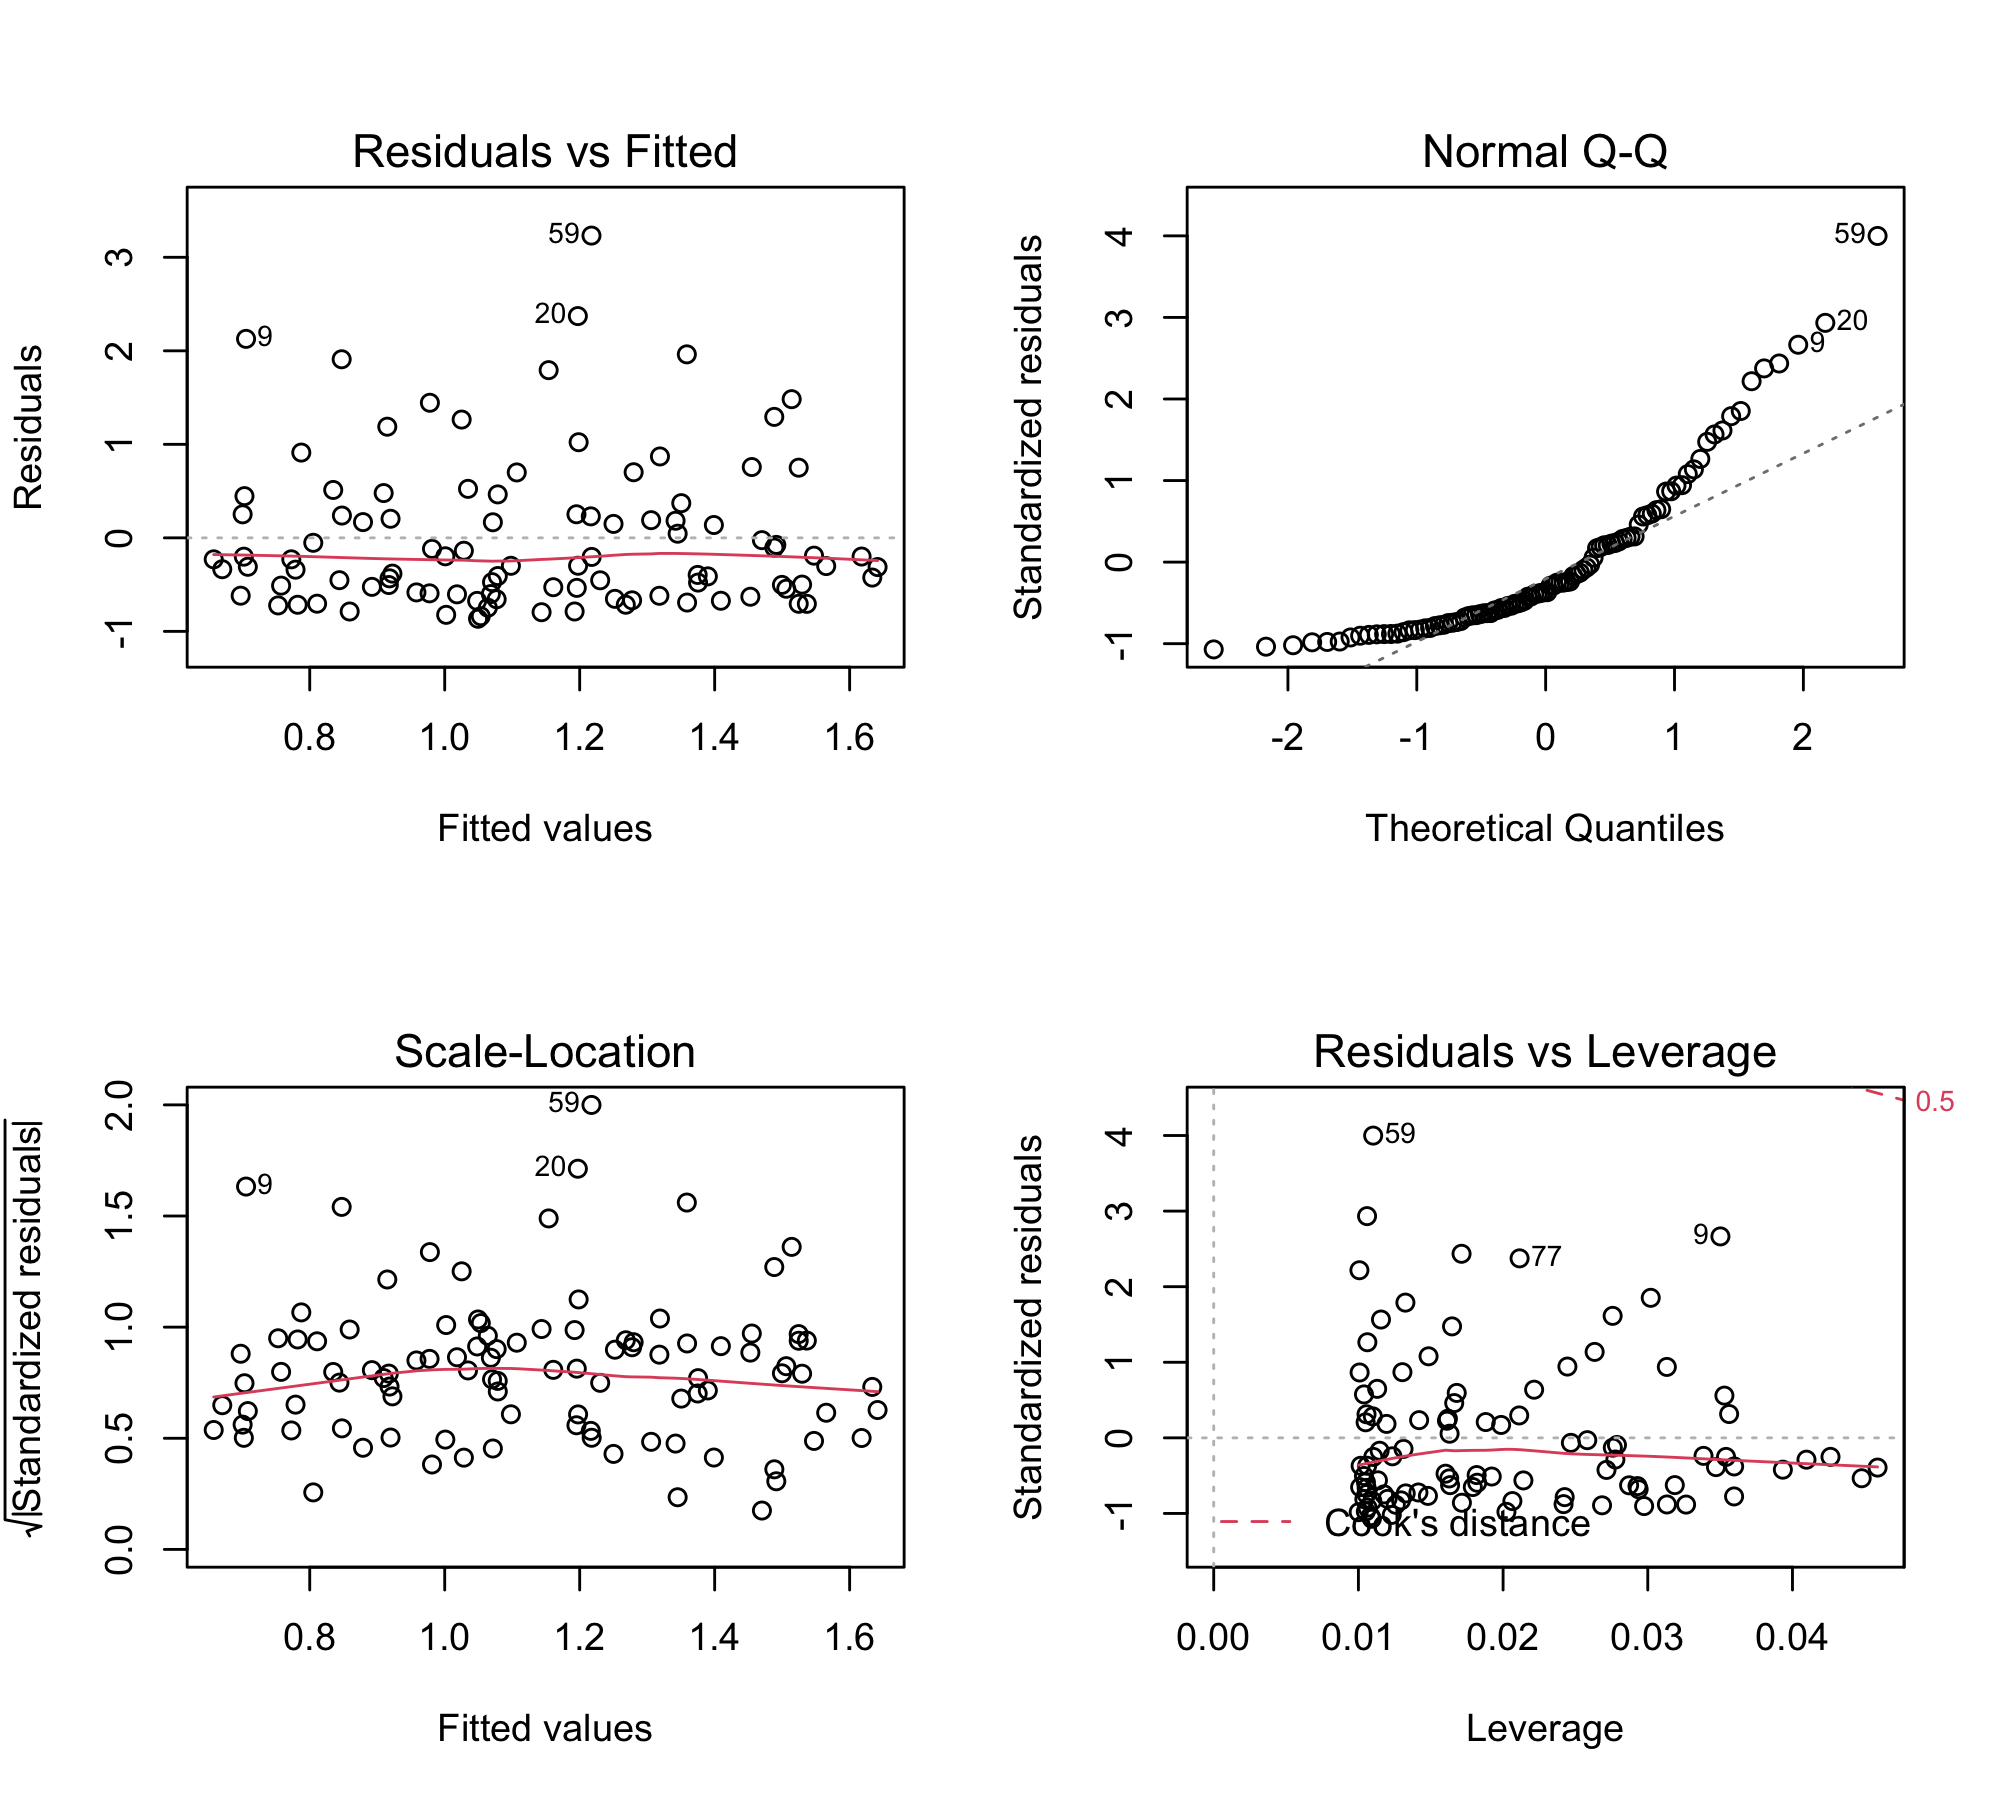
\includegraphics[scale=0.23]{extras/plots_df2}
				\captionof{figure}{Plots of the Function \ref{eq:2} without transformations}
				\label{fig:lr_df2}
			\end{center}
		\end{figure}

		Then, Figure  \ref{fig:max_likelihood} shows a Maximum Likelihood plot for the values of $\lambda$ with a 95\% confidence interval. This plot gives a threshold with bounds of the recommended $\lambda$ values for the Box-Cox transformation. Then the best value can be extracted, which represents the value when the curve is higher. This threshold can be seen by simple inspection; it moves from 0.1 to 0.5 approximately. Finally, the calculated value of $\lambda$ is 0.263.

		\begin{figure}
			\begin{center}
				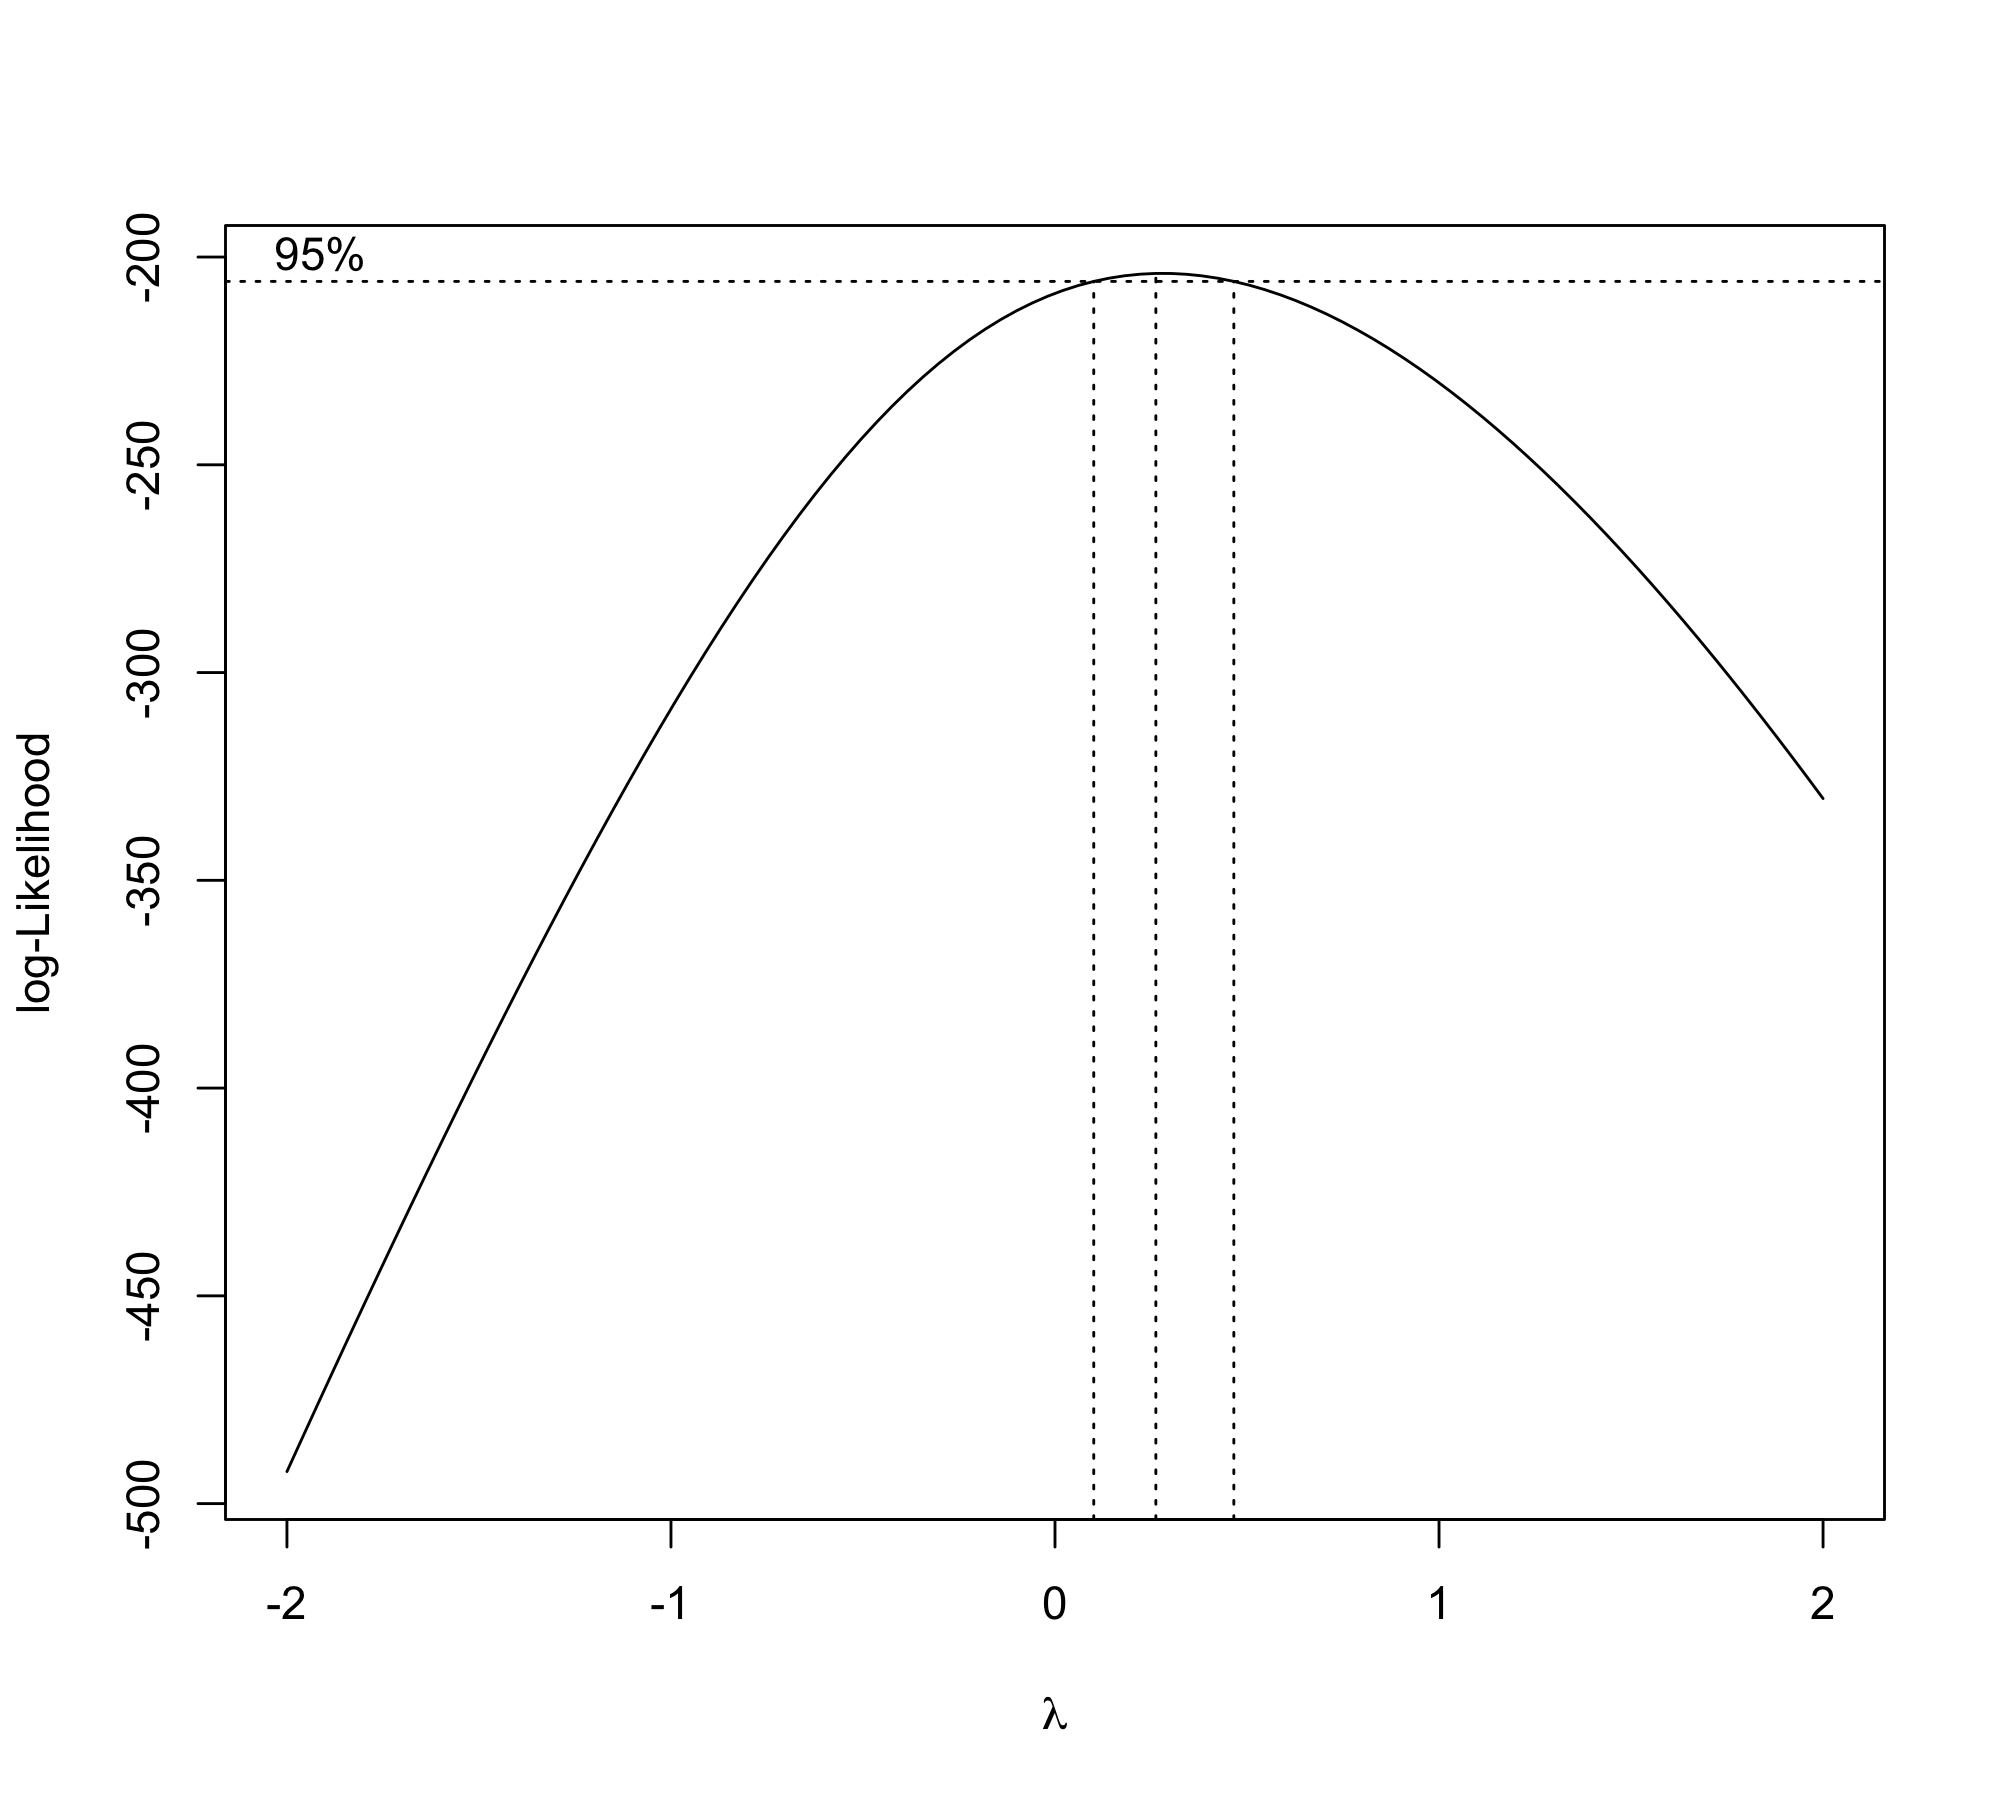
\includegraphics[scale=0.20]{extras/likelihood}
				\captionof{figure}{Max-Likelihood plot to determine the best $\lambda$ for the Box-Cox Transformation}
				\label{fig:max_likelihood}
			\end{center}
		\end{figure}

		Figure \ref{eq:2} represents the same model diagnosis, but after performing the Box-Cox transformation with the previously calculated parameter, $\lambda$=0.263. Here main changes can be appreciated in the ``$QQ$ Plot, which shows a better approximation to the normal line.

		\begin{figure}
		\begin{center}
			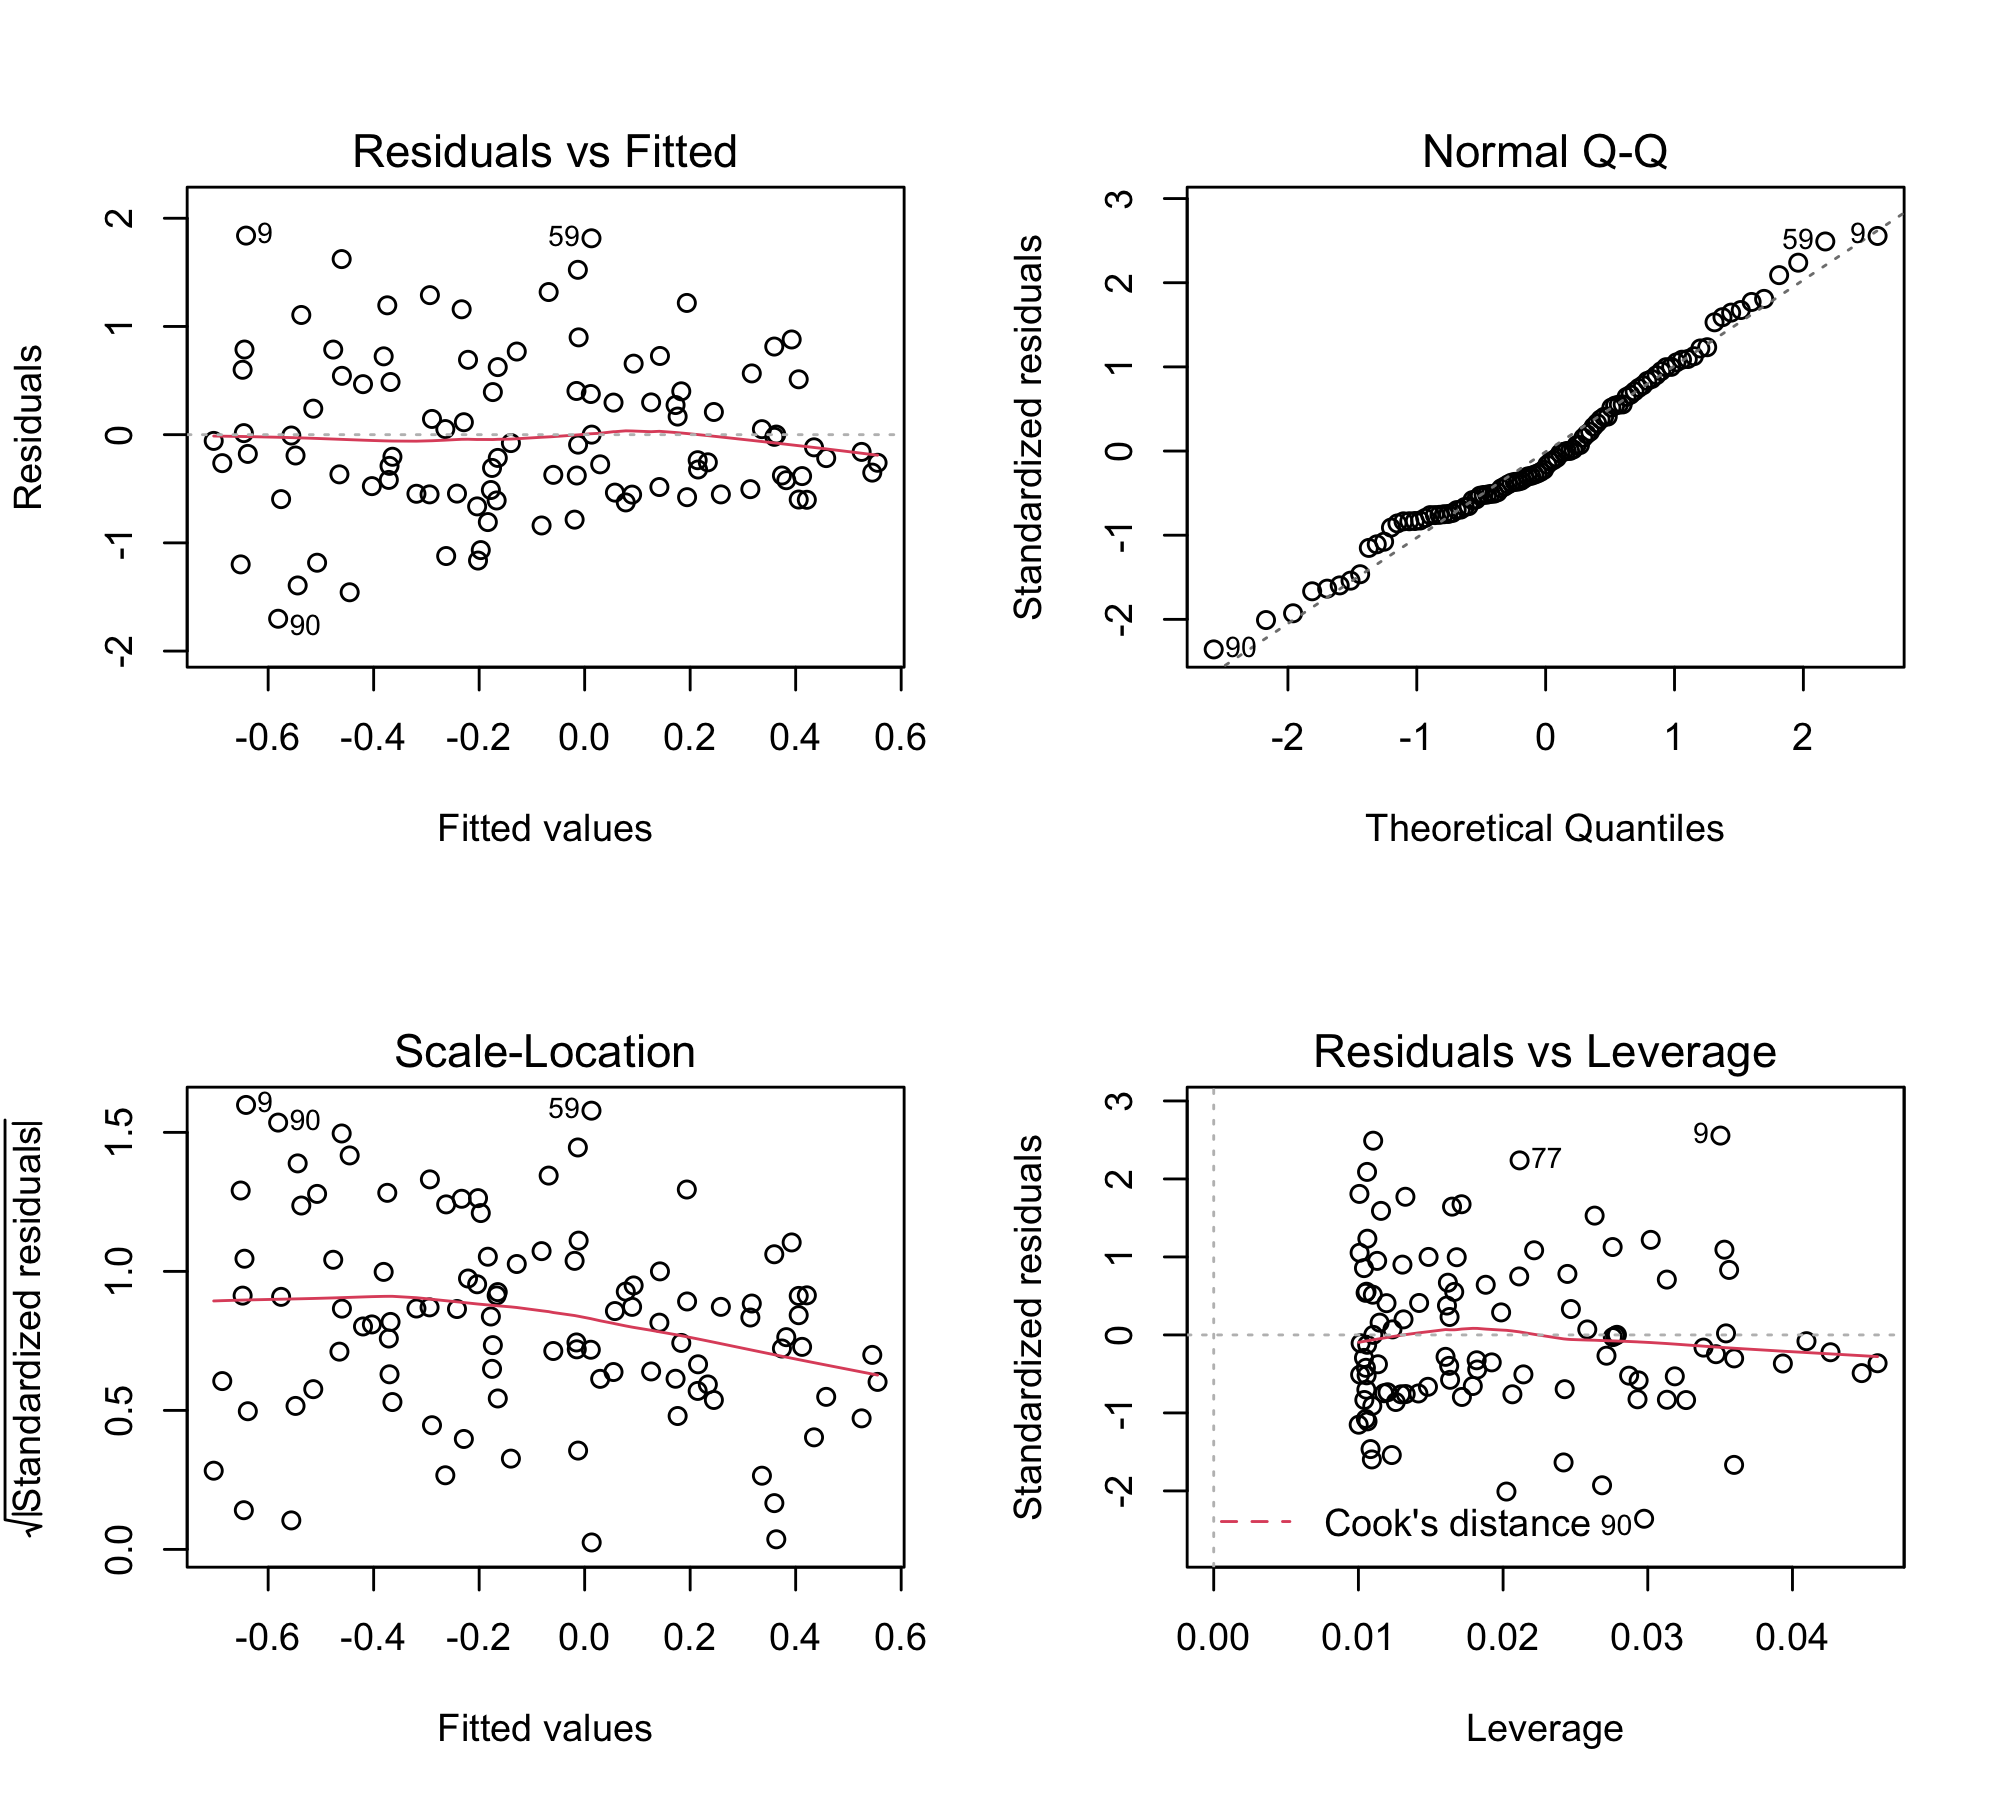
\includegraphics[scale=0.23]{extras/boxcox}
			\captionof{figure}{Plots of the Function \ref{eq:2} using the Box-Cox Transformation}
			\label{fig:boxcox_df2}
		\end{center}
	\end{figure}
		
\begin{comment}

	\subsection{Multivariate Analysis of Variance}
	
	The analysis in this section, requires a multivariate distribution by dealing with outcomes that have different combinaton of explanatory varaibles \citep{MATHEW198930}. In this case Function \eqref{eq:3} represents the outcomes of two treatments, so it is needed a bivariate distribution .

		\VerbatimInput{extras/manova_eq3.txt}
\end{comment}

	\subsection{Log Transformation}

		Log transformations are another method that can be valuable for making patterns in the data more interpretable and for helping to meet the assumptions of inferential statistics \cite{lane2003introduction}. This log transformation it is used in Function \ref{eq:4}, which depends of the variables $x_{1}$ and $ x_{2} $.

		\VerbatimInput{extras/log.txt}
		
		In the R output show for this section, the logarithm's coefficient for each independent variable and the intercept's value can be seen.
		
		\subsection{Tukey's Ladder of Power}
		
		\citet{tukey1977exploratory} describes an orderly way of re-expressing variables using a power transformation suggesting exploring simple relationships such as $ y^{\lambda} = b_{0} + b_{1}X $ where $\lambda$ is a parameter chosen to make the relationship as close to a straight line as possible. Table \ref{tab:ladders} show examples of the Tukey's ladder of transformations.
		
			\VerbatimInput{extras/tukey.txt}
			
			In the above output corresponding to the \texttt{transformTukey()} function of R, applied to Function \ref{eq:2} it shows the value of $\lambda$which data could be transformed, which is $\lambda = 0.675$ and the transformation should be $x^\lambda$. Figure \ref{fig:tukey} shows a histogram of the transformation.
			
			\begin{figure}
				\begin{center}
					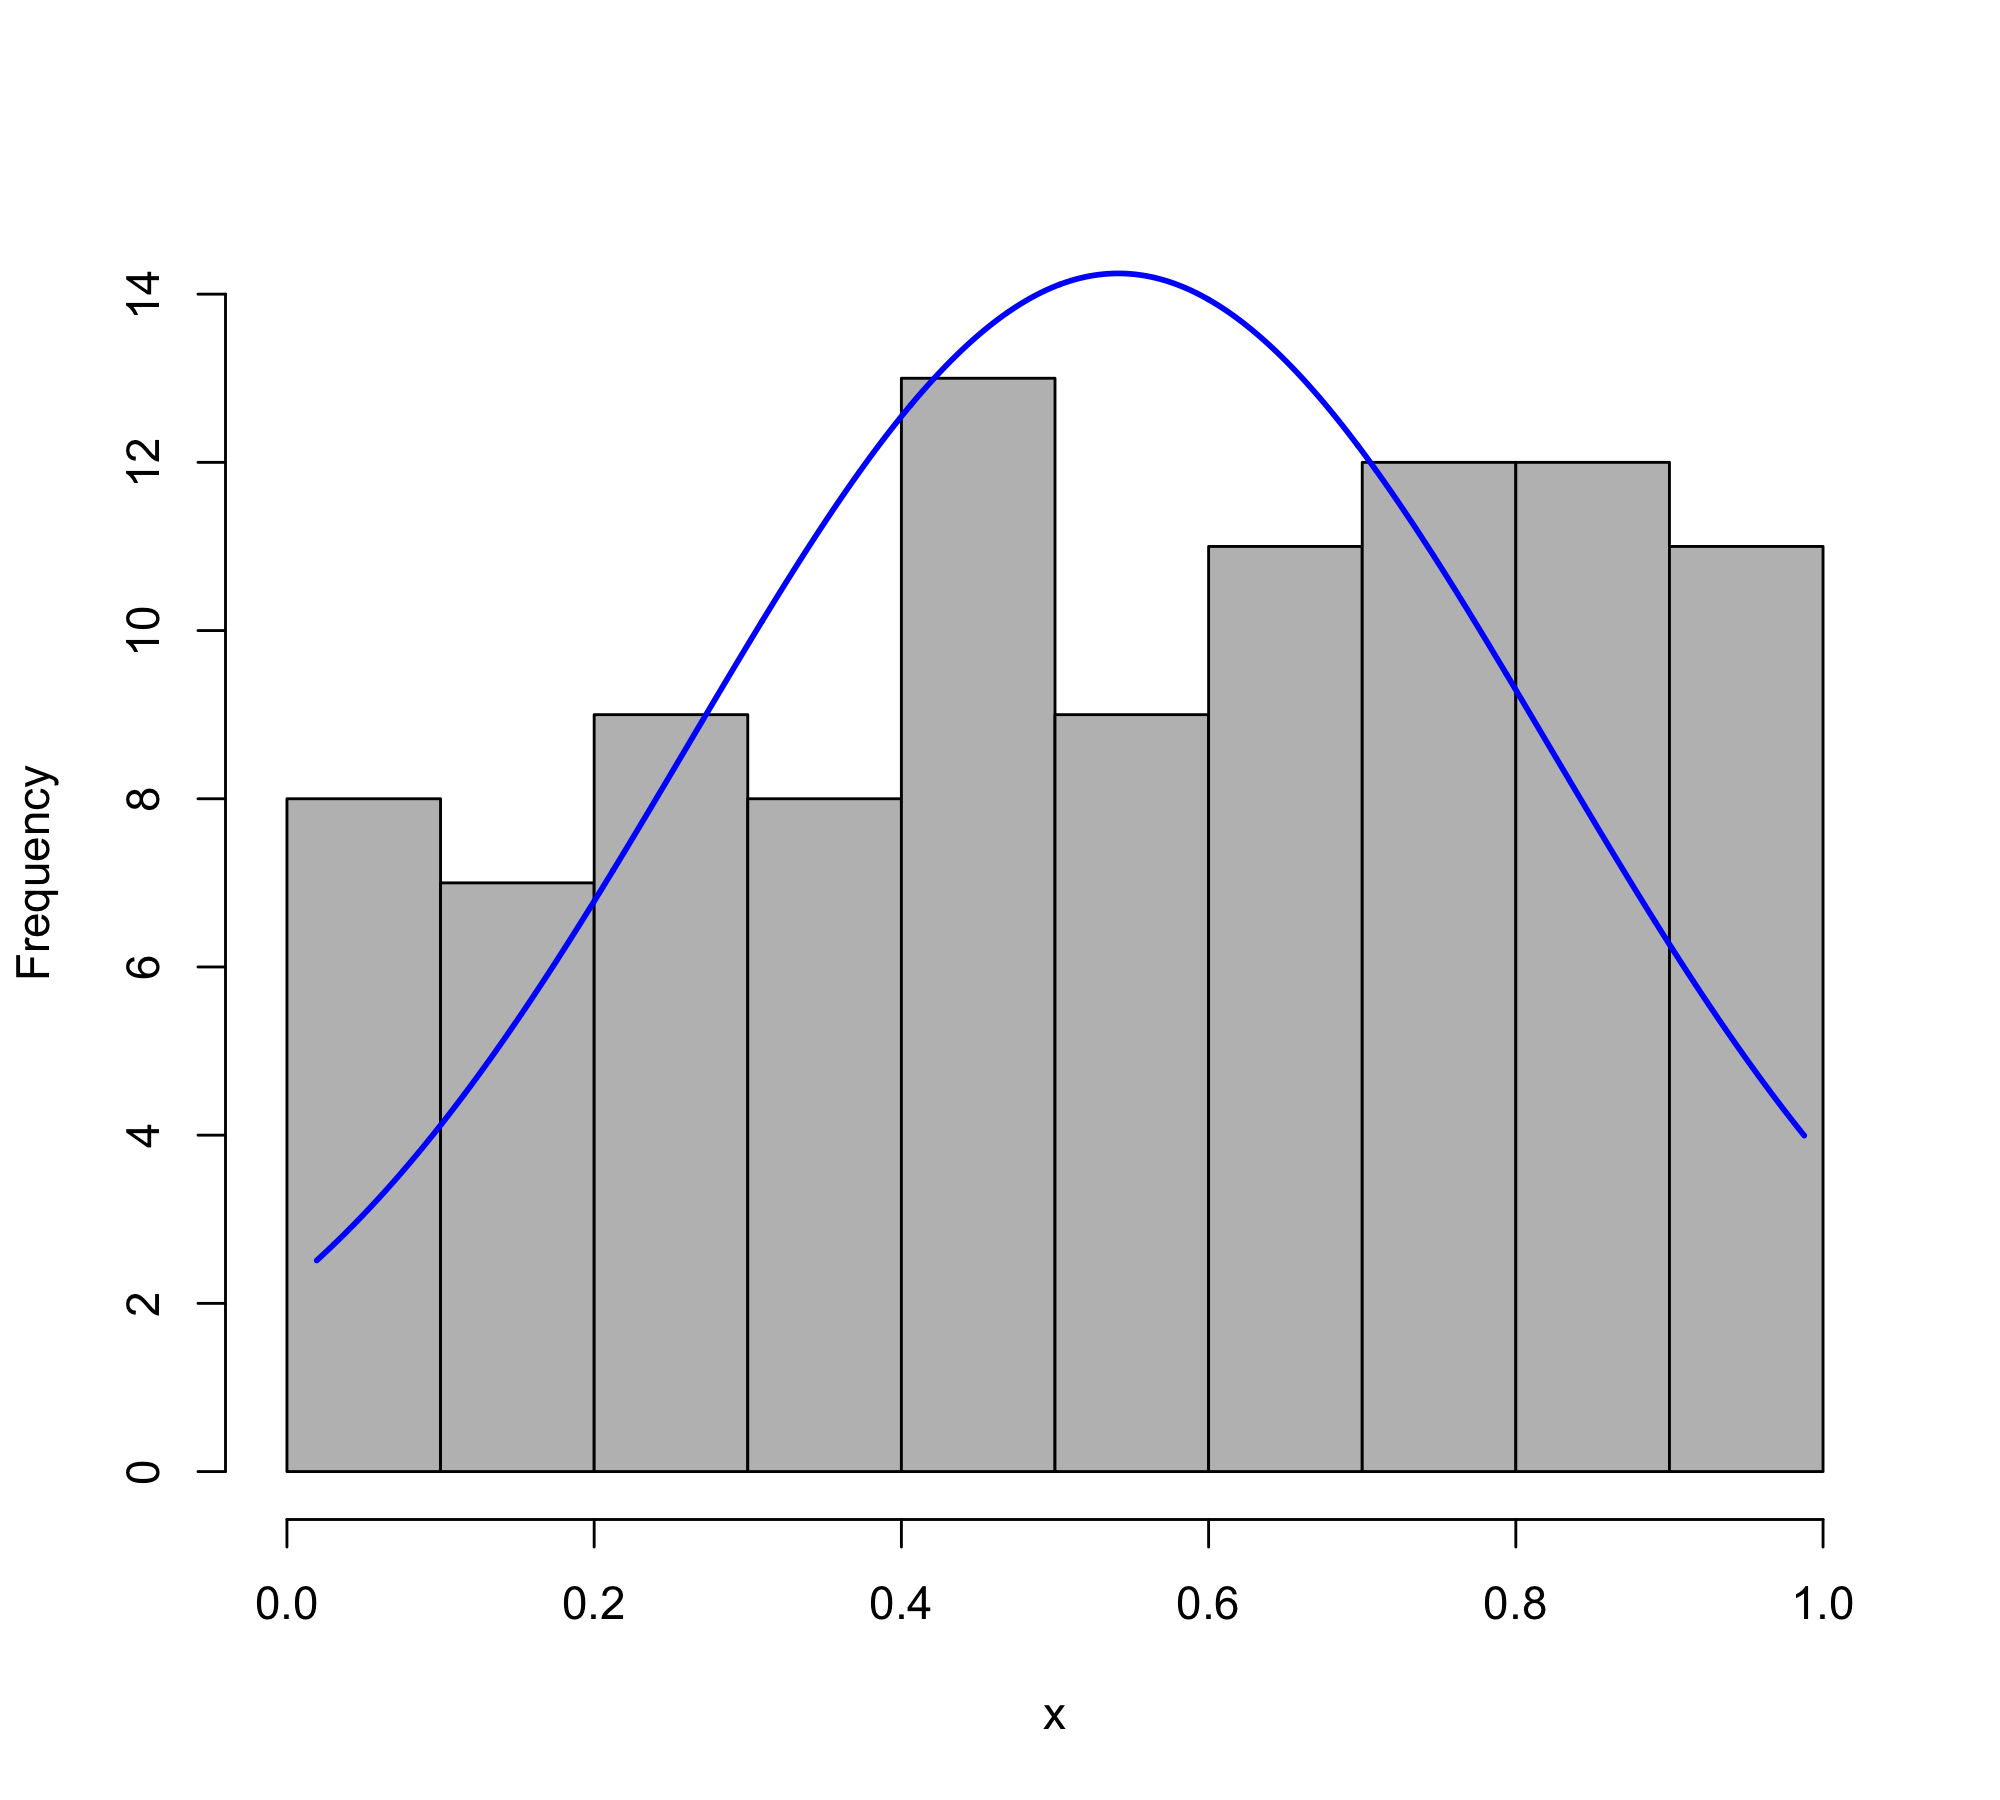
\includegraphics[scale=0.15]{extras/tukeyimg}
					\captionof{figure}{Histogram of Function \ref{eq:2} using the Tukey Ladder  of Power Transformation}
					\label{fig:tukey}
				\end{center}
			\end{figure}			
		
		% Please add the following required packages to your document preamble:
		% \usepackage{booktabs}
		\begin{table}[]
			\centering
			\caption{Tukey's Ladder of Transformations}
			\label{tab:ladders}
			\begin{tabular}{@{}|l|ccccccc|@{}}
				\toprule
				\textbf{$\lambda$} & -2                & -1            & -$\dfrac{1}{2}$      & 0       & $\dfrac{1}{2}$ & 1   & 2       \\ \midrule
				\textbf{$y$}       & $\dfrac{1}{x^{2}}$ & $\dfrac{1}{x}$ & $\dfrac{1}{\sqrt{x}}$ & $\log x$ & $\sqrt{x}$     & $x$ & $x^{2}$ \\ \bottomrule
			\end{tabular}
		\end{table}

	\subsection{Stepwise Regression}

		The stepwise regression (or stepwise selection) consists of iteratively adding and removing predictors in the predictive model to find the subset of variables in the data set, resulting in the best performing model, that is, a model that lowers prediction error \citep{kassambara2018stepwise}. 
		
		Here a comparison of the resulting fit model of multiple linear regression with the stepwise regression is performed. The R output showed below shows the results of fitting data applying multiple linear regression, indicating the intercept and values of the coefficient of all $x$ variables.
		
		%\vspace{5cm}
		\VerbatimInput{extras/mlr.txt}

		This last R output shows the final model results by performing the stepwise regression, where it can be seen it removes variables $x_{3} $ and $ x_{4} $ from the initial model to predict $y$, in contrast with the multiple linear regression. Finally, it can be expressed the final models resulting form this two methods in Table \ref{tab:models}.
		
		\VerbatimInput{extras/stepwise.txt}
		
		
			
		% Please add the following required packages to your document preamble:
		% \usepackage{booktabs}
		\begin{table}[]
			\centering
			\caption{Resulting Models from the two methods for Function \ref{eq:5}}
			\label{tab:models}
			\begin{tabular}{@{}cc@{}}
				\toprule
				\textbf{Multiple Linear Regression Model} & \textbf{Stepwise Regression Model} \\ \midrule
				    $31.81x_{1 }   + 20.02x_{2} - 0.25x_{3}    + 0.32x_{4 } - 16.96$    &           $43.49 x_{1}  + 26.48x_{2} - 27.09$ \\  \bottomrule
			\end{tabular}
		\end{table}
		
\clearpage

	\bibliography{assignment7}
	\bibliographystyle{plainnat}
	
\end{document}